% <-- a percent symbol indicates a comment which does not affect the output of LaTeX
% you can leave the preamble alone, from here ...
\documentclass[12pt]{article}

\usepackage{amssymb,amsmath,amsthm}
\usepackage{tikz}
\usepackage[top=1in, bottom=1in, left=1.25in, right=1.25in]{geometry}
\usepackage{enumitem,palatino}
\usepackage[colorlinks=true,citecolor=blue,linkcolor=red,urlcolor=blue]{hyperref}

\newtheorem{problem}{Problem}
% ... to here

% shortcuts for blackboard bold number sets (reals, integers, etc.)
\newcommand{\II}{\ensuremath{\mathbb I}}
\newcommand{\NN}{\ensuremath{\mathbb N}}
\newcommand{\QQ}{\ensuremath{\mathbb Q}}
\newcommand{\RR}{\ensuremath{\mathbb R}}
\newcommand{\ZZ}{\ensuremath{\mathbb Z}}
\newcommand{\PP}{\ensuremath{\mathbb{P}}}

\newcommand{\eps}{\ensuremath{\epsilon}}
\newcommand{\ds}{\displaystyle}

% feel free to add more shortcuts here


\begin{document}
% replace with your name, but otherwise leave this header alone, from here ...
\small
\noindent \textsc{Math F307: Homework Assignment 2} \hfill Christopher Munoz

\normalsize
\bigskip
% ... to here
\section*{Section 1.4: Sets}


\setcounter{problem}{1}
\begin{problem}
Let $A = \{1, 2, 3\}$, $B = \{n \in \PP : n \text{ is even}\}$, and $C = \{n \in \PP : n \text{ is odd}\}$.
\begin{enumerate}[label=(\alph*)]
    \item Determine $A \cap B$, $B \cap C$, $B \cup C$, and $B \oplus C$.
    
    \item List all subsets of $A$.
    
    \item Which of the following sets are infinite? $A \oplus B$, $A \oplus C$, $A \setminus C$, $C \setminus A$.
\end{enumerate}
\end{problem}

\begin{proof}[Solution]
~
\begin{enumerate}[label=(\alph*)]
    \item $B = \{2, 4, 6, 8, \ldots\}$ (even positive integers) and $C = \{1, 3, 5, 7, \ldots\}$ (odd positive integers).
    
    $A \cap B = \{2\}$ 
    
    $B \cap C = \emptyset$ 
    
    $B \cup C = \PP$ 
    
    $B \oplus C = (B \cup C) \setminus (B \cap C) = \PP \setminus \emptyset = \PP$ 
    
    \item The subsets of $A$ are:
    $$\emptyset, \{1\}, \{2\}, \{3\}, \{1,2\}, \{1,3\}, \{2,3\}, \{1,2,3\}$$
    
    \item $A \oplus B = (A \cup B) \setminus (A \cap B) = \{1, 3, 4, 6, 8, \ldots\}$ - infinite
  
    $A \oplus C = (A \cup C) \setminus (A \cap C) = \{5, 7, 9, 11, \ldots\}$ - infinite
    
    $A \setminus C = \{2\}$ - finite
    
    $C \setminus A = \{5, 7, 9, 11, \ldots\}$ - infinite

\end{enumerate}
\end{proof}



\setcounter{problem}{5}
\begin{problem}
The following statements about sets are false. For each statement, give an example, i.e., a choice of sets, for which the statement is false. Such examples are called counterexamples. They are examples that are counter to, i.e., contrary to, the assertion.
\begin{enumerate}[label=(\alph*)]
    \item $A \cup B \subseteq A \cap B$ for all $A$, $B$.
    
    \item $A \cap \emptyset = A$ for all $A$.
    
    \item $A \cap (B \cup C) = (A \cap B) \cup C$ for all $A$, $B$, $C$.
\end{enumerate}
\end{problem}

\begin{proof}[Solution]
~
\begin{enumerate}[label=(\alph*)]
    \item \textbf{Counterexample:} Let $A = \{1\}$ and $B = \{2\}$.
    
    Then $A \cup B = \{1, 2\}$ and $A \cap B = \emptyset$.
    
    But $\{1, 2\} \not\subseteq \emptyset$, so the statement is false.
    
    \item \textbf{Counterexample:} Let $A = \{1, 2, 3\}$.
    
    Then $A \cap \emptyset = \emptyset \neq \{1, 2, 3\} = A$, so the statement is false.
    
    (In fact, $A \cap \emptyset = \emptyset$ for all sets $A$.)
    
    \item \textbf{Counterexample:} Let $A = \{1\}$, $B = \{2\}$, $C = \{3\}$.
    
    Then $A \cap (B \cup C) = \{1\} \cap \{2, 3\} = \emptyset$.
    
    But $(A \cap B) \cup C = \emptyset \cup \{3\} = \{3\}$.
    
    Since $\emptyset \neq \{3\}$, the statement is false.

\end{enumerate}
\end{proof}



\setcounter{problem}{7}
\begin{problem}
For the sets $A = \{1, 3, 5, 7, 9, 11\}$ and $B = \{2, 3, 5, 7, 11\}$, determine the following numbers.
\begin{enumerate}[label=(\alph*)]
    \item $|A|$
    
    \item $|B|$
    
    \item $|A \cup B|$
    
    \item $|A| + |B| - |A \cap B|$
    
    \item Do you see a general reason why the answers to (c) and (d) have to be the same?
\end{enumerate}
\end{problem}

\begin{proof}[Solution]
~
\begin{enumerate}[label=(\alph*)]
    \item $|A| = 6$ (counting: 1, 3, 5, 7, 9, 11)
    
    \item $|B| = 5$ (counting: 2, 3, 5, 7, 11)
    
    \item $A \cap B = \{3, 5, 7, 11\}$, so $|A \cap B| = 4$
    
    $A \cup B = \{1, 2, 3, 5, 7, 9, 11\}$, so $|A \cup B| = 7$
    
    \item $|A| + |B| - |A \cap B| = 6 + 5 - 4 = 7$
    
    \item When we count $|A| + |B|$, we count every element in $A \cap B$ twice (once for being in $A$, once for being in $B$). Subtracting by the intersection of $A$ and $B$ removes the copy elements.

\end{enumerate}
\end{proof}



\setcounter{problem}{9}
\begin{problem}
\begin{enumerate}[label=(\alph*)]
    \item Show that relative complementation is not commutative; that is, the equality $A \setminus B = B \setminus A$ can fail.
    
    \item Show that relative complementation is not associative: $(A \setminus B) \setminus C = A \setminus (B \setminus C)$ can fail.
\end{enumerate}
\end{problem}

\begin{proof}[Solution]
~
\begin{enumerate}[label=(\alph*)]
    \item \textbf{Counterexample:} Let $A = \{1, 2\}$ and $B = \{2, 3\}$.
    
    Then $A \setminus B = \{1\}$ (elements in $A$ but not in $B$).
    
    And $B \setminus A = \{3\}$ (elements in $B$ but not in $A$).
    
    Since $\{1\} \neq \{3\}$, we have $A \setminus B \neq B \setminus A$.
    
    Therefore, relative complementation is not commutative.
    
    \item \textbf{Counterexample:} Let $A = \{1, 2, 3\}$, $B = \{2\}$, $C = \{3\}$.
    
    $(A \setminus B) \setminus C = (\{1, 2, 3\} \setminus \{2\}) \setminus \{3\} = \{1, 3\} \setminus \{3\} = \{1\}$
    
    $A \setminus (B \setminus C) = \{1, 2, 3\} \setminus (\{2\} \setminus \{3\}) = \{1, 2, 3\} \setminus \{2\} = \{1, 3\}$
    
    Since $\{1\} \neq \{1, 3\}$, we have $(A \setminus B) \setminus C \neq A \setminus (B \setminus C)$.
    
    Therefore, relative complementation is not associative.

\end{enumerate}
\end{proof}



\setcounter{problem}{11}
\begin{problem}
Let $S = \{0, 1, 2, 3, 4\}$ and $T = \{0, 2, 4\}$.
\begin{enumerate}[label=(\alph*)]
    \item How many ordered pairs are in $S \times T$? $T \times S$?
    \setcounter{enumi}{2}
    
    \item List or draw the elements in the set $\{(m, n) \in T \times S : m < n\}$.
    \setcounter{enumi}{4}
    
    \item List or draw the elements in the set $\{(m, n) \in T \times S : mn > 4\}$.
\end{enumerate}
\end{problem}

\begin{proof}[Solution]
~
\begin{enumerate}[label=(\alph*)]
    \item $|S \times T| = |S| \cdot |T| = 5 \cdot 3 = 15$ ordered pairs
    
    $|T \times S| = |T| \cdot |S| = 3 \cdot 5 = 15$ ordered pairs
    
    \setcounter{enumi}{2}
    
    \item $\{(m, n) \in T \times S : m < n\}$ where $T = \{0, 2, 4\}$ and $S = \{0, 1, 2, 3, 4\}$:
    
    For $m = 0$: $(0,1), (0,2), (0,3), (0,4)$
    
    For $m = 2$: $(2,3), (2,4)$
    
    For $m = 4$: none (no element in $S$ is greater than 4)
    
    Answer: $\{(0,1), (0,2), (0,3), (0,4), (2,3), (2,4)\}$
    
    \setcounter{enumi}{4}
    
    \item $\{(m, n) \in T \times S : mn > 4\}$:
    
    For $m = 0$: $0 \cdot n = 0 \not> 4$ for all $n$
    
    For $m = 2$: $2 \cdot 3 = 6 > 4$ and $2 \cdot 4 = 8 > 4$, so $(2,3), (2,4)$
    
    For $m = 4$: $4 \cdot 2 = 8 > 4$, $4 \cdot 3 = 12 > 4$, $4 \cdot 4 = 16 > 4$, so $(4,2), (4,3), (4,4)$
    
    Answer: $\{(2,3), (2,4), (4,2), (4,3), (4,4)\}$

\end{enumerate}
\end{proof}



\section*{Section 1.5: Functions}

\setcounter{problem}{1}
\begin{problem}
Consider the function $h: \PP \to \PP$ defined by $h(n) = |\{k \in \NN : k \mid n\}|$ for $n \in \PP$. In words, $h(n)$ is the number of divisors of $n$. Calculate $h(n)$ for $1 \leq n \leq 10$ and for $n = 73$.

(Note: In this textbook, $\PP = \ZZ^+ = \{1, 2, 3, 4, \ldots\}$)
\end{problem}

\begin{proof}[Solution]
We count the divisors of each number:

\begin{align*}
h(1) &= 1 \quad \text{(divisors: 1)} \\
h(2) &= 2 \quad \text{(divisors: 1, 2)} \\
h(3) &= 2 \quad \text{(divisors: 1, 3)} \\
h(4) &= 3 \quad \text{(divisors: 1, 2, 4)} \\
h(5) &= 2 \quad \text{(divisors: 1, 5)} \\
h(6) &= 4 \quad \text{(divisors: 1, 2, 3, 6)} \\
h(7) &= 2 \quad \text{(divisors: 1, 7)} \\
h(8) &= 4 \quad \text{(divisors: 1, 2, 4, 8)} \\
h(9) &= 3 \quad \text{(divisors: 1, 3, 9)} \\
h(10) &= 4 \quad \text{(divisors: 1, 2, 5, 10)} \\
h(73) &= 2 \quad \text{(divisors: 1, 73, since 73 is prime)}
\end{align*}

\end{proof}



\begin{problem}[Section 1.5 Extra \#1]
  Suppose that $f : \ZZ \to \ZZ$ by $n \mapsto \lfloor \frac{n}{2} \rfloor$ and $g : \ZZ \to \ZZ$ by $n \mapsto 3n$.

Draw portions of arrow diagrams representing each of the four functions $f$, $g$, $f \circ g$, and $g \circ f$.

You need to make sure you include enough integers so it's clear what's going on.

\textit{Example:} If $h : n \mapsto 2n + 3$, I can represent that with an arrow diagram as follows:

\begin{center}
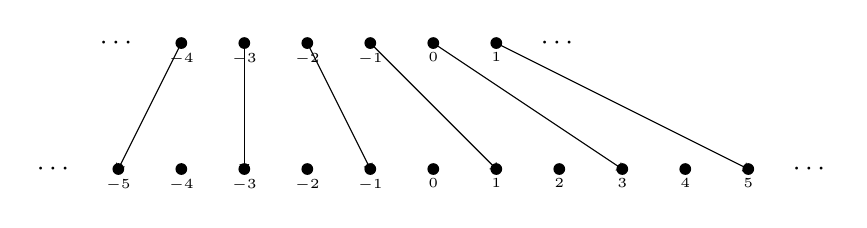
\begin{tikzpicture}[scale=0.8]
% Domain
\foreach \x in {-4,-3,-2,-1,0,1} {
    \node[circle,fill,inner sep=1.5pt] at (\x, 0) {};
    \node[below] at (\x, 0) {\tiny $\x$};
}
\node at (-5, 0) {$\cdots$};
\node at (2, 0) {$\cdots$};

% Codomain
\foreach \y in {-5,-4,-3,-2,-1,0,1,2,3,4,5} {
    \node[circle,fill,inner sep=1.5pt] at (\y, -2) {};
    \node[below] at (\y, -2) {\tiny $\y$};
}
\node at (-6, -2) {$\cdots$};
\node at (6, -2) {$\cdots$};

% Arrows
\draw[->] (-4,0) -- (-5,-2);
\draw[->] (-3,0) -- (-3,-2);
\draw[->] (-2,0) -- (-1,-2);
\draw[->] (-1,0) -- (1,-2);
\draw[->] (0,0) -- (3,-2);
\draw[->] (1,0) -- (5,-2);
\end{tikzpicture}
\end{center}
\end{problem}

\begin{proof}[Solution]
~

\textbf{Function $f : \ZZ \to \ZZ$ by $n \mapsto \lfloor n/2 \rfloor$:}

\begin{center}
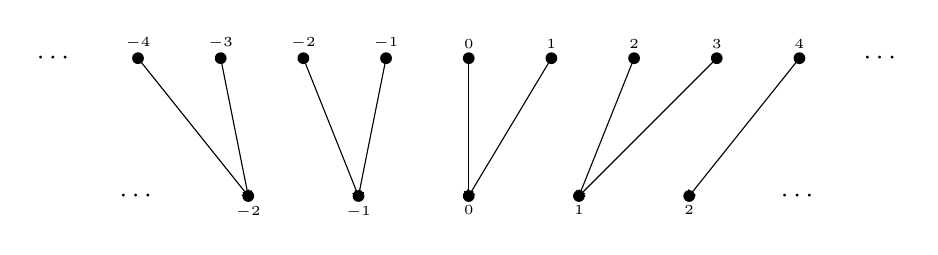
\begin{tikzpicture}[scale=0.7]
% Domain
\foreach \x in {-4,-3,-2,-1,0,1,2,3,4} {
    \node[circle,fill,inner sep=1.5pt] at (1.5*\x, 0) {};
    \node[above] at (1.5*\x, 0) {\tiny $\x$};
}
\node at (-7.5, 0) {$\cdots$};
\node at (7.5, 0) {$\cdots$};

% Codomain
\foreach \y in {-2,-1,0,1,2} {
    \node[circle,fill,inner sep=1.5pt] at (2*\y, -2.5) {};
    \node[below] at (2*\y, -2.5) {\tiny $\y$};
}
\node at (-6, -2.5) {$\cdots$};
\node at (6, -2.5) {$\cdots$};

% Arrows
\draw[->] (-6,0) -- (-4,-2.5);   % -4 -> -2
\draw[->] (-4.5,0) -- (-4,-2.5); % -3 -> -2
\draw[->] (-3,0) -- (-2,-2.5);   % -2 -> -1
\draw[->] (-1.5,0) -- (-2,-2.5); % -1 -> -1
\draw[->] (0,0) -- (0,-2.5);     % 0 -> 0
\draw[->] (1.5,0) -- (0,-2.5);   % 1 -> 0
\draw[->] (3,0) -- (2,-2.5);     % 2 -> 1
\draw[->] (4.5,0) -- (2,-2.5);   % 3 -> 1
\draw[->] (6,0) -- (4,-2.5);     % 4 -> 2
\end{tikzpicture}
\end{center}

\vspace{0.5in}

\textbf{Function $g : \ZZ \to \ZZ$ by $n \mapsto 3n$:}

\begin{center}
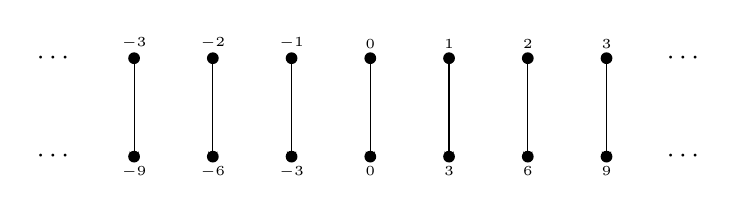
\begin{tikzpicture}[scale=0.5]
% Domain
\foreach \x in {-3,-2,-1,0,1,2,3} {
    \node[circle,fill,inner sep=1.5pt] at (2*\x, 0) {};
    \node[above] at (2*\x, 0) {\tiny $\x$};
}
\node at (-8, 0) {$\cdots$};
\node at (8, 0) {$\cdots$};

% Codomain
\foreach \y in {-9,-6,-3,0,3,6,9} {
    \node[circle,fill,inner sep=1.5pt] at (\y/1.5, -2.5) {};
    \node[below] at (\y/1.5, -2.5) {\tiny $\y$};
}
\node at (-8, -2.5) {$\cdots$};
\node at (8, -2.5) {$\cdots$};

% Arrows
\draw[->] (-6,0) -- (-6,-2.5);   % -3 -> -9
\draw[->] (-4,0) -- (-4,-2.5);   % -2 -> -6
\draw[->] (-2,0) -- (-2,-2.5);   % -1 -> -3
\draw[->] (0,0) -- (0,-2.5);     % 0 -> 0
\draw[->] (2,0) -- (2,-2.5);     % 1 -> 3
\draw[->] (4,0) -- (4,-2.5);     % 2 -> 6
\draw[->] (6,0) -- (6,-2.5);     % 3 -> 9
\end{tikzpicture}
\end{center}

\newpage

\textbf{Function $f \circ g : \ZZ \to \ZZ$ by $n \mapsto f(g(n)) = f(3n) = \lfloor 3n/2 \rfloor$:}

\begin{center}
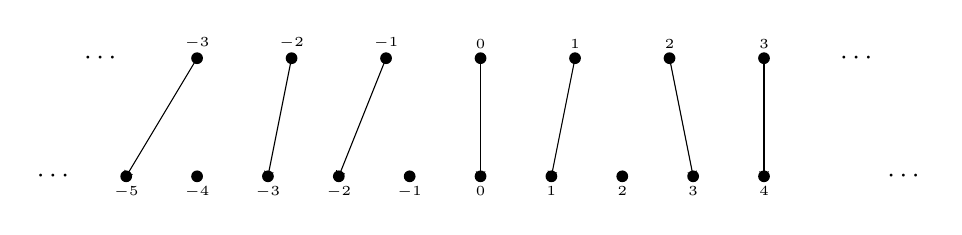
\begin{tikzpicture}[scale=0.6]
% Domain
\foreach \x in {-3,-2,-1,0,1,2,3} {
    \node[circle,fill,inner sep=1.5pt] at (2*\x, 0) {};
    \node[above] at (2*\x, 0) {\tiny $\x$};
}
\node at (-8, 0) {$\cdots$};
\node at (8, 0) {$\cdots$};

% Codomain
\foreach \y in {-5,-4,-3,-2,-1,0,1,2,3,4} {
    \node[circle,fill,inner sep=1.5pt] at (1.5*\y, -2.5) {};
    \node[below] at (1.5*\y, -2.5) {\tiny $\y$};
}
\node at (-9, -2.5) {$\cdots$};
\node at (9, -2.5) {$\cdots$};

% Arrows
\draw[->] (-6,0) -- (-7.5,-2.5); % -3 -> -5
\draw[->] (-4,0) -- (-4.5,-2.5); % -2 -> -3
\draw[->] (-2,0) -- (-3,-2.5);   % -1 -> -2
\draw[->] (0,0) -- (0,-2.5);     % 0 -> 0
\draw[->] (2,0) -- (1.5,-2.5);   % 1 -> 1
\draw[->] (4,0) -- (4.5,-2.5);   % 2 -> 3
\draw[->] (6,0) -- (6,-2.5);     % 3 -> 4
\end{tikzpicture}
\end{center}

\vspace{0.5in}

\textbf{Function $g \circ f : \ZZ \to \ZZ$ by $n \mapsto g(f(n)) = g(\lfloor n/2 \rfloor) = 3\lfloor n/2 \rfloor$:}

\begin{center}
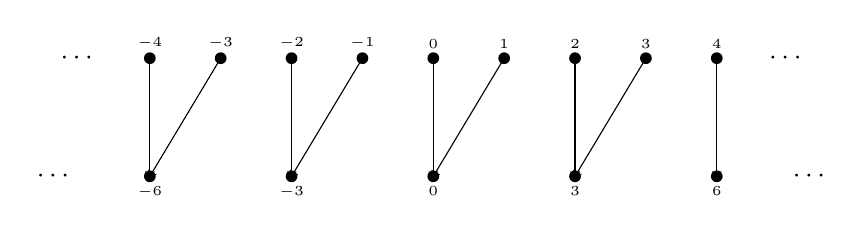
\begin{tikzpicture}[scale=0.6]
% Domain
\foreach \x in {-4,-3,-2,-1,0,1,2,3,4} {
    \node[circle,fill,inner sep=1.5pt] at (1.5*\x, 0) {};
    \node[above] at (1.5*\x, 0) {\tiny $\x$};
}
\node at (-7.5, 0) {$\cdots$};
\node at (7.5, 0) {$\cdots$};

% Codomain
\foreach \y in {-6,-3,0,3,6} {
    \node[circle,fill,inner sep=1.5pt] at (\y/1, -2.5) {};
    \node[below] at (\y/1, -2.5) {\tiny $\y$};
}
\node at (-8, -2.5) {$\cdots$};
\node at (8, -2.5) {$\cdots$};

% Arrows
\draw[->] (-6,0) -- (-6,-2.5);   % -4 -> -6
\draw[->] (-4.5,0) -- (-6,-2.5); % -3 -> -6
\draw[->] (-3,0) -- (-3,-2.5);   % -2 -> -3
\draw[->] (-1.5,0) -- (-3,-2.5); % -1 -> -3
\draw[->] (0,0) -- (0,-2.5);     % 0 -> 0
\draw[->] (1.5,0) -- (0,-2.5);   % 1 -> 0
\draw[->] (3,0) -- (3,-2.5);     % 2 -> 3
\draw[->] (4.5,0) -- (3,-2.5);   % 3 -> 3
\draw[->] (6,0) -- (6,-2.5);     % 4 -> 6
\end{tikzpicture}
\end{center}

\end{proof}

\section*{Section 1.6: Sequences}

\setcounter{problem}{1}
\begin{problem}
Simplify:
\begin{enumerate}[label=(\alph*)]
    \item $\frac{n!}{(n-1)!}$
    
    \item $\frac{(n!)^2}{(n+1)!(n-1)!}$
\end{enumerate}
\end{problem}

\begin{proof}[Solution]
~
\begin{enumerate}[label=(\alph*)]
    \item $\frac{n!}{(n-1)!} = \frac{n \cdot (n-1)!}{(n-1)!} = n$
    
    \item $\frac{(n!)^2}{(n+1)!(n-1)!} = \frac{(n!)^2}{(n+1) \cdot n! \cdot (n-1)!} = \frac{n! \cdot n!}{(n+1) \cdot n! \cdot (n-1)!} = \frac{n!}{(n+1)(n-1)!}$
    
    $= \frac{n \cdot (n-1)!}{(n+1)(n-1)!} = \frac{n}{n+1}$
\end{enumerate}

\end{proof}



\setcounter{problem}{3}
\begin{problem}
Calculate:
\begin{enumerate}[label=(\alph*)]
    \setcounter{enumi}{3}
    \item $\prod_{n=1}^{5} (2n+1)$
    
    \item $\prod_{j=4}^{8} (j-1)$
\end{enumerate}
\end{problem}

\begin{proof}[Solution]
~
\begin{enumerate}[label=(\alph*)]
    \setcounter{enumi}{3}
    \item $\prod_{n=1}^{5} (2n+1) = (2 \cdot 1 + 1)(2 \cdot 2 + 1)(2 \cdot 3 + 1)(2 \cdot 4 + 1)(2 \cdot 5 + 1)$
    
    $= (3)(5)(7)(9)(11) = 10{,}395$
    
    \item $\prod_{j=4}^{8} (j-1) = (4-1)(5-1)(6-1)(7-1)(8-1)$
    
    $= (3)(4)(5)(6)(7) = 2{,}520$
\end{enumerate}
\end{proof}



\setcounter{problem}{5}
\begin{problem}
\begin{enumerate}[label=(\alph*)]
    \item Calculate $\sum_{k=0}^{n} 2^k$ for $n = 1, 2, 3, 4$, and $5$.
    
    \item Use your answers to part (a) to guess a general formula for this sum.
\end{enumerate}
\end{problem}

\begin{proof}[Solution]
~
\begin{enumerate}[label=(\alph*)]
    \item 
    \begin{align*}
    n = 1: \quad \sum_{k=0}^{1} 2^k &= 2^0 + 2^1 = 1 + 2 = 3 \\
    n = 2: \quad \sum_{k=0}^{2} 2^k &= 2^0 + 2^1 + 2^2 = 1 + 2 + 4 = 7 \\
    n = 3: \quad \sum_{k=0}^{3} 2^k &= 1 + 2 + 4 + 8 = 15 \\
    n = 4: \quad \sum_{k=0}^{4} 2^k &= 1 + 2 + 4 + 8 + 16 = 31 \\
    n = 5: \quad \sum_{k=0}^{5} 2^k &= 1 + 2 + 4 + 8 + 16 + 32 = 63
    \end{align*}
    
    \item Looking at the pattern:
    \begin{align*}
    n = 1: & \quad 3 = 4 - 1 = 2^2 - 1 = 2^{1+1} - 1 \\
    n = 2: & \quad 7 = 8 - 1 = 2^3 - 1 = 2^{2+1} - 1 \\
    n = 3: & \quad 15 = 16 - 1 = 2^4 - 1 = 2^{3+1} - 1 \\
    n = 4: & \quad 31 = 32 - 1 = 2^5 - 1 = 2^{4+1} - 1 \\
    n = 5: & \quad 63 = 64 - 1 = 2^6 - 1 = 2^{5+1} - 1
    \end{align*}
    
    \textbf{General formula:} $\sum_{k=0}^{n} 2^k = 2^{n+1} - 1$
\end{enumerate}
\end{proof}



\setcounter{problem}{9}
\begin{problem}
For $n = 1, 2, 3, \ldots$, let $\text{SSQ}(n) = \sum_{i=1}^{n} i^2$.
\begin{enumerate}[label=(\alph*)]
    \item Calculate $\text{SSQ}(n)$ for $n = 1, 2, 3$, and $5$.
    
    \item Observe that $\text{SSQ}(n + 1) = \text{SSQ}(n) + (n + 1)^2$ for $n \geq 1$.
    
    \item It turns out that $\text{SSQ}(73) = 132{,}349$. Use this to calculate $\text{SSQ}(74)$ and $\text{SSQ}(72)$.
\end{enumerate}
\end{problem}

\begin{proof}[Solution]
~
\begin{enumerate}[label=(\alph*)]
    \item 
    \begin{align*}
    \text{SSQ}(1) &= 1^2 = 1 \\
    \text{SSQ}(2) &= 1^2 + 2^2 = 1 + 4 = 5 \\
    \text{SSQ}(3) &= 1^2 + 2^2 + 3^2 = 1 + 4 + 9 = 14 \\
    \text{SSQ}(5) &= 1^2 + 2^2 + 3^2 + 4^2 + 5^2 = 1 + 4 + 9 + 16 + 25 = 55
    \end{align*}
    
    \item This follows from the definition: 
    $$\text{SSQ}(n+1) = \sum_{i=1}^{n+1} i^2 = \sum_{i=1}^{n} i^2 + (n+1)^2 = \text{SSQ}(n) + (n+1)^2$$
    
    \item Given $\text{SSQ}(73) = 132{,}349$:
    
    $\text{SSQ}(74) = \text{SSQ}(73) + 74^2 = 132{,}349 + 5{,}476 = 137{,}825$
    
    For $\text{SSQ}(72)$, we use: $\text{SSQ}(73) = \text{SSQ}(72) + 73^2$
    
    So $\text{SSQ}(72) = \text{SSQ}(73) - 73^2 = 132{,}349 - 5{,}329 = 127{,}020$
\end{enumerate}
\end{proof}

\begin{problem}[Section 1.6 Extra \#1]
Go to the Online Encyclopedia of Integer Sequences, \url{http://oeis.org}, and find an interesting sequence. Write down the sequence, explain a little about the definition of the sequence, and say why you think it is interesting.
\end{problem}

\begin{proof}[Solution]
~

\textbf{Sequence:} The Kolakoski Sequence (OEIS A000002)

$$1, 2, 2, 1, 1, 2, 1, 2, 2, 1, 2, 2, 1, 1, 2, 1, 1, 2, 2, 1, 2, 1, 1, 2, 1, 2, 2, 1, \ldots$$

\textbf{Definition:}

The Kolakoski sequence is the unique sequence of 1's and 2's that is its own run-length encoding. That is, if you read the sequence and count the lengths of consecutive runs of the same symbol, you get the sequence itself back.

More precisely:
\begin{itemize}
\item The sequence starts with 1, 2, 2
\item The first element (1) tells us the first run has length 1, so we have one 1
\item The second element (2) tells us the second run has length 2, so we have two 2's: 1, 2, 2
\item The third element (2) tells us the third run has length 2, so we have two 1's: 1, 2, 2, 1, 1
\item The fourth element (1) tells us the fourth run has length 1, so we have one 2: 1, 2, 2, 1, 1, 2
\item And so on...
\end{itemize}

On top of the sequence itself being interesting, the discoverer William Kolakoski himself is also an interesting figure, an artist mathematician plagued by schizophrenia. Although the sequence was named after him, it was actually discovered in 1939 by Rufus Oldenburger though it wasn't noticed at the time. It is also the second sequence in the OEIS database.
\end{proof}

\end{document}
